% Chapter Template
\chapter{Approaches} % Main chapter title

\label{ch:03} %

The normal inference task involves estimating the surface normal of a 3D object, assuming that the surface of the object is mathematically unknown. This means that we cannot simply use the cross product of two non-parallel surface vectors to find the normal. Instead, the surface is sensed by digital sensors under certain types of data, which can be divided into two groups. The first group is geometry data, where a point cloud is used to capture the geometry information of the surface in 3D space. The approach that uses point clouds for normal estimation is called geometry-based approach.
Another type of data is images that record the reflectance and shading of the surface under the following lighting conditions. The surface normal is calculated based on specific light models such as BRDF. The other approach, which uses the relationship between reflectance and shading to calculate the surface normal, is called photometric stereo.

In this chapter, the geometric and photometric stereo based approaches are presented separately. Then, a method for estimating the surface normal using both types of data based on deep learning approaches is introduced.





\section{Notations}

In the following chapters of this thesis the following standard notations are used. The bold capital letters stand for matrices, while the bold lowercase letters stand for vectors. The Greek capital letters stand for planes.
The subscript $ i= \{1,2,...\} $ stands for the index of observations, the superscript for the dimension of the matrices or vectors, e.g. $ \textbf{n}^{3\times 1} $ for a vector of dimension $ 3\times 1 $. We use $ W $ for the width, $ H $ for the height and $ C $ for the number of channels.


\section{Geometry-based Normal Estimation}

Geometry-based normal estimation uses the point cloud of the object surface as input. The task can be formulated as follows.

Given a structured point cloud $ \textbf{V}^{W\times H\times 3} $, in which the 3D point positions are stored with respect to the image grid. We want to compute the corresponding normal map $ \textbf{N}^{W\times H \times 3} $. The normal map is simply a matrix representation of the normals of all points in the point cloud. A normal $ \textbf{n}^{3\times 1} $ at the point $ \textbf{p}^{3\times 1} \in \textbf{V} $ is a unit vector whose direction is outward from the surface and perpendicular to the tangent plane of the surface at point $ \textbf{p} $.


The idea behind the neighborhood-based method is to fit a plane $ \tilde\Pi $ containing the $ k $ neighbors $ \textbf{p}_1, ..., \textbf{p}_k \in \mathbb{R}^{3\times1} $ of the point $ \textbf{p} $, then compute the normal $ \tilde{\textbf{n}} $ of the plane $ \tilde\Pi $. The $ \tilde{\textbf{n}} $ is considered as an approximation to the normal $ \textbf{n} $ of the tangent plane $ \Pi $.

The point and its neighbors are assumed to lie in the same plane $ \Pi $, which is exactly the tangent plane of the surface at the point $\textbf{p} $. 
This is usually not true for most of the surface, since the surface is usually not flat, but has some degree of curvature. But if $ k $ is of a suitable scale and the point cloud is dense enough, we can approximately consider all $ k $ neighboring points in a small area on the same tangent plane. Then we have an approximation $ \textbf{n} \approx \tilde{\textbf{n}}$, where $ \tilde{\textbf{n}}$ denotes the estimated normal. Similarly, the estimated tangent plane $ \tilde{\Pi} \approx \Pi $. 


Based on the above assumption, the task of normal inference is trivial, since the surface is then mathematically describable. We can generate the approximate tangent plane at each point with its neighbors, then the normal $ \tilde{\textbf{n}} $ of the tangent plane can be derived from the following equations.

\[\tilde{\textbf{n}} \cdot \textbf{v}_{ij} = 0 \]
where 
\[ \textbf{v}_{ij} = \textbf{p}_i - \textbf{p}_j, \text{for } i, j \in \{ 1,2,...,k\}, i\neq j \]
To find a normal, we need at least 3 neighbors that are not on the same line to solve the above equation. Calculate the normal for each point on the point cloud, then we can get the corresponding normal maps. 

If we consider more than 3 neighbors, the points are usually not on the same plane. In this case, the system of equations is overdetermined. We can use the optimization approach to find a plane that has the least distance to all points in 3D space. By $ \textbf{A }\in \mathbb{R}^{k\times 3} $ we denote the vector matrix vertically stacked by the $ k $ vectors we found on the approximated tangent surface. Then the system of equations is transformed into an optimization problem 



\begin{equation}
	\begin{array}{rrclcl}
		\displaystyle \min & \multicolumn{3}{l}{\|\textbf{ A}  \bn \|^2_2} \\
		\\
		\textrm{s.t.} & \| \bn \|^2_2 & = & 1 
	\end{array}
\end{equation}
where the additional condition is added to avoid trivial solutions, and the normal is supposed to be a unit vector.

The above problem can be solved by singular value decomposition (SVD), where.
\[ \textbf{A}= \textbf{U}\boldmath{\Sigma} \textbf{V}^T \]
The last column of $ \textbf{V} $ is the solution of the system of equations and consequently the surface normal. 

The optimization based approach using SVD is more robust compared to selecting only 3 points for normal computation, since the plane generated by 3 neighbors is not guaranteed to be a good approximation to the actual tangent plane. However, the size of the neighbors $ k $ is a key parameter of this approach. For the smooth surface, a relatively larger $ k $ can help the system of equations find a plane that is closer to the tangent plane. For the sharp surface, $ k $ must be small enough to ensure that the points it contains are still approximately in the same plane, otherwise the more points it contains will just be the outliers for the equation solution. 

Finally, after solving the above equation, we should convert all normals to the viewpoint $ \textbf{s} $ for uniformity. Thus, the direction of a normal should be inverted if 


\begin{equation}\label{eq:normal-invertion}
	\textbf{n} \cdot (\textbf{p}  - \textbf{s}) > 0
\end{equation}
Since the above approach is essentially solved by SVD, this method will be referred to as \textit{SVD} in the remainder of the paper for simplicity.

\section{Photometric Stereo based Normal Estimation}
Photometric stereo was originally introduced by \cite{photometric-stereo} and is a completely different approach from the geometry information based approach such as \textit{SVD}. It estimates the surface normal of the object by observing the object in the same position under different illuminated conditions. It is based on the fact that the light reflected from a surface depends on the surface normal and the light direction.

Before presenting this approach, let us discuss what we can actually obtain from the images.
An image $ \textbf{I} $ can be decomposed into two parts: the reflectance $ \textbf{R} $ and the shading $ \textbf{S} $,
\[ \textbf{I} = \textbf{R}\odot \textbf{S}\]
where $ \odot $ denotes the element-wise product. This decomposition of the image is based on the intrinsic image model proposed by \cite{intrinsic-image}. It interprets the observed image into a reflection image and a shading image. Figure \ref{fig:intrinsic-image} shows a visualization of the decomposition.

%% insert an image for decompositions
\begin{figure}[th]
	\centering
	\captionsetup{width=\linewidth}
	{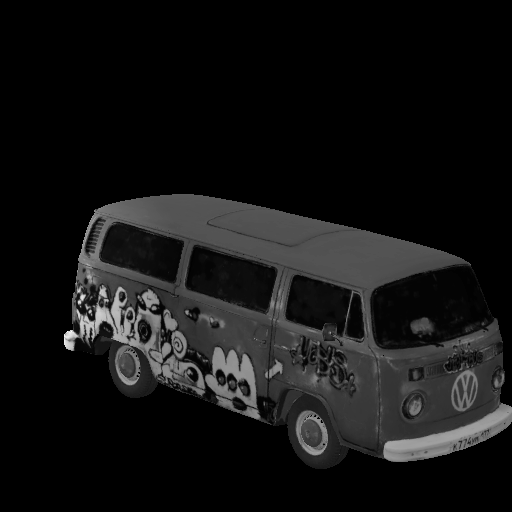
\includegraphics[width=.19\textwidth]{./Figures/intrinsic_image.png}}
	{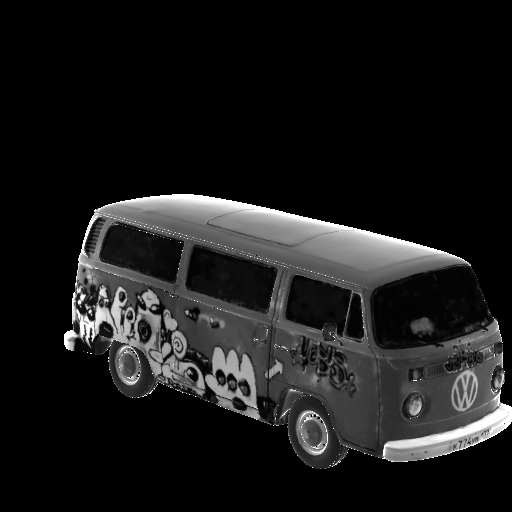
\includegraphics[width=.19\textwidth]{./Figures/intrinsic_image_reflectance.png}}
	{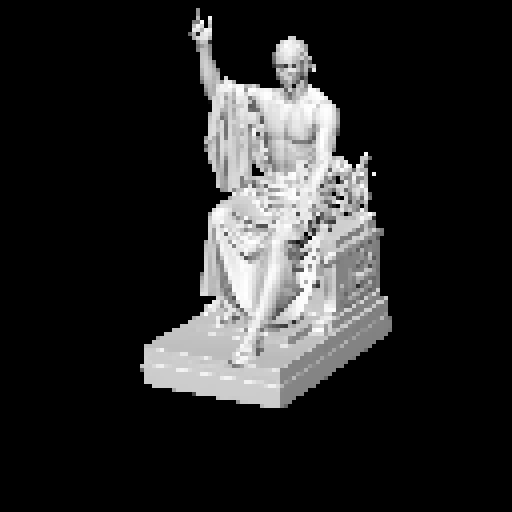
\includegraphics[width=.19\textwidth]{./Figures/intrinsic_image_shading.png}}
	{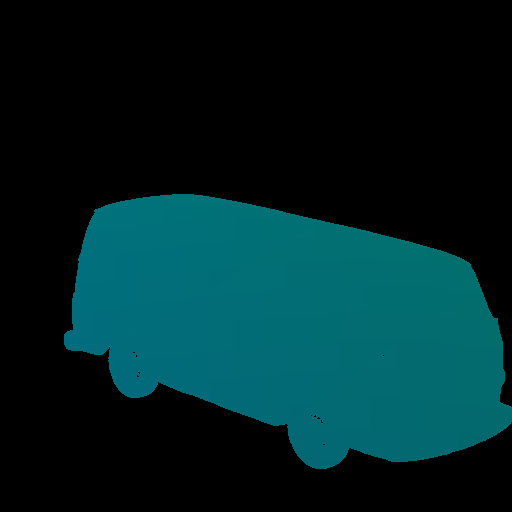
\includegraphics[width=.19\textwidth]{./Figures/intrinsic_image_light.png}}
	{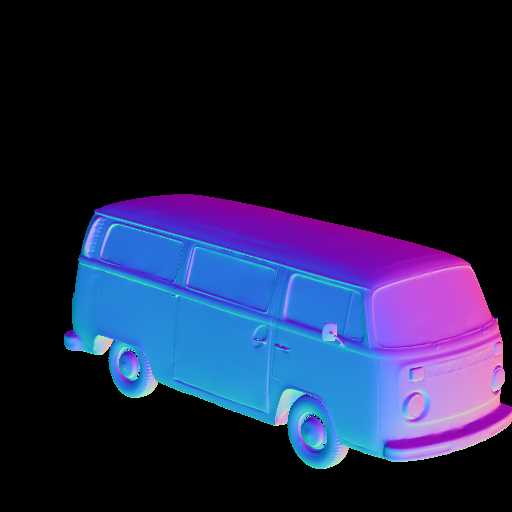
\includegraphics[width=.19\textwidth]{./Figures/intrinsic_image_normal.png}}
	\decoRule
	\caption{Intrinsic image analysis of the Washington object. From left to right: original image, reflection image, shading image, light image, normal image.}
	\label{fig:intrinsic-image}
	
\end{figure}

The equation can be further decomposed based on different surface models. If we assume that the object surfaces are Lambertian surfaces, i.e. surfaces that reflect light in all directions, as shown in Figure \ref{fig:lambertian-surface}, then the reflectance is equal to the albedo $ \rho $, the shading image can be decomposed as the product of the radiance of the incident light $ L_0 $ and the cosine of the angle of incidence, which is the dot product of the surface normal $ \textbf{N} $ and the light source direction $ \textbf{L} $.
\[ \textbf{I} = \rho \odot ( L_0 \textbf{L} \cdot \textbf{N}) \]
Note that each surface normal in the matrix $ \textbf{N} $ and each light direction in the matrix $ \textbf{L} $ is a unit vector, so they have only two degrees of freedom. 


\begin{figure}[th]
	\centering
	\captionsetup{width=\linewidth}
	\begin{subfigure}[b]{0.49\linewidth}
		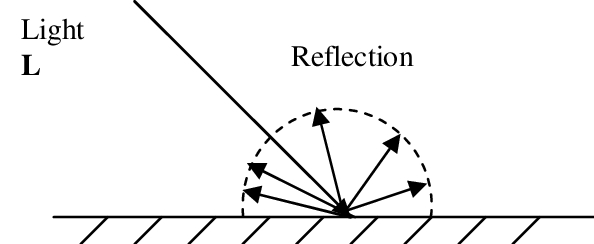
\includegraphics[width=\textwidth]{./Figures/Lambertian-Reflection-Lambertian-Surface.png}
	\end{subfigure}
	\begin{subfigure}[b]{0.49\linewidth}
		\begin{tikzpicture} 
			% reference lines
			\coordinate (light) at (-1,3);
			\coordinate (p) at (2,0);
			\coordinate (normal) at (2,3);
			\draw [fill=blue!20] plot [smooth cycle] coordinates {(0,0) (1,1) (3,1) (5,0) (2,-1)}; %% surface element
			\draw[thick, ->] (2,0) -- (2,3) node[midway, left] {$ \textbf{n} $}; %% normal
			\draw[thick, ->] (2,0) -- (-1,3) node[midway, left] {$ \textbf{l} $}  ; %% source direction
			\pic [draw, ->, "$\theta$", angle eccentricity=1.5] {angle = normal--p--light};
			\draw[thick, ->] (2,0) -- (5,3) node[midway, left] {$ \textbf{v} $}; %% view direction
			\filldraw[black] (-1,3) circle (2pt) node[anchor=south west]{light source}; %% light source
			\filldraw[black] (5,3) circle (2pt) node[anchor=south west]{view point}; %% view point		
		\end{tikzpicture}
	\end{subfigure}
	\decoRule
	\caption{Left: the reflection of light on a Lambertian surface. (Image source \cite{lambertian-reflectance}). Right: the surface normal, the light direction of the source and the viewing direction, where $ \theta $ denotes the angle between the light direction and the normal.}
	\label{fig:lambertian-surface}
\end{figure}
The equation can be rearranged as follows
\[ \textbf{I} =(L_0\rho \odot \textbf{N}) \cdot ( \textbf{L}) \]
Let $ \textbf{G} =L_0\rho \odot \textbf{N} $, the equation simplifies to
\[\textbf{I} = \textbf{G} \cdot \textbf{L}\]
If we use a set of $ k $ images for the same scene, taken based on different light projections. Then, for each pixel $ (x,y) $ in a scene, we can set up a system of equations 

\[ 
\begin{pmatrix}
	\textbf{l}_1^T \\
	\textbf{l}_2^T \\
	\cdots \\
	\textbf{l}_k^T
\end{pmatrix} \textbf{G}(x,y) = 
\begin{pmatrix}
	\textbf{I}_1(x,y) \\
	\textbf{I}_2(x,y) \\
	\cdots \\
	\textbf{I}_k(x,y)
\end{pmatrix}
\]
For simplicity, $ \textbf{l}_i^T $ for $ 1\le i \le k $ denotes the direction of light at position $ (x,y) $ in $ k $-th image . The equation can be solved using the least squares method. Then, the albedo can be determined with the light intensity, since the normal is a unit vector,

\[ \| \textbf{G}(x,y)\|_2 = \|L_0\rho(x,y)\textbf{N}(x,y)\|_2 = L_0\rho(x,y) \]
Then the normal can be determined as follows

\[ \textbf{N}(x,y) = \frac{\textbf{G}(x,y)}{L_0\rho(x,y)}\]
We compute the surface normal for each point to obtain the surface normal map. 

This approach is also called Shape from Shading (\textit{SFS}) \cite{SFS}. Both normal maps and the corresponding albedo are obtained from a series of images under different lighting conditions. Since the direction of light is used in the calculation, the cameras and the position of the light source must be calibrated beforehand. 

In the shape from shading approach, at least three light positions are considered for normal estimation on a pixel. It is also common to use more than three light sources to cover most points of the surface as much as possible. 

We assume that in each neighborhood there is a coherent behavior for the albedo that can be modeled by the filters in the neural network, and in the following section we propose an learning based approach for normal inference from geometry information, but using only one illuminated scene.


\newpage 
\section{Gated Convolution Neural Network for Surface Normal Estimation}
\label{sec:gcnn}

Recently, Deep Learning based methods have achieved great success in image processing\cite{yolov3} \cite{efficientDet}. These network architectures use a stack of RGB/grayscale images as input and are used for classification problems. Typically, the images are convolved with convolutional layers and sampled with pooling layers. The output values of the networks consist of a single value representing the index of the corresponding class, or a set of values representing the position of the bounding boxes\cite{yolov3}. However, in many other image processing tasks, such as inference of normal maps, the output is required to have the same form as the input, while each pixel in the output image requires a prediction. Therefore, the output consists not only of one or several labels, but of a matrix similar in size to the input. In this case, the traditional network architecture with full connections in the last layers is no longer suitable for label prediction.

%% talk about image upsampling, unet
\cite{unet} has proposed an architecture called \textit{U-Net} for biomedical image segmentation. The architecture is shown in Figure \ref{fig:u-net}. This net has a very regular architecture for data processing, while the down/up sampling part has a similar design. For the feature extraction part, called down-sampling, the architecture follows the traditional CNN architecture. For the up-sampling part, the network uses an architecture similar to the down-sampling operations, which uses the same convolutional operations but replaces the max-pool layers with up-conv layers. An important design is the skip connection in the up-sampling part. The feature maps extracted in the down-sampling part are concatenated with the feature maps in the up-sampling part. This helps the network to find the locations in the original image and use them to predict a sharp output.

\begin{figure}[th]
	\centering
	\captionsetup{width=\linewidth}
	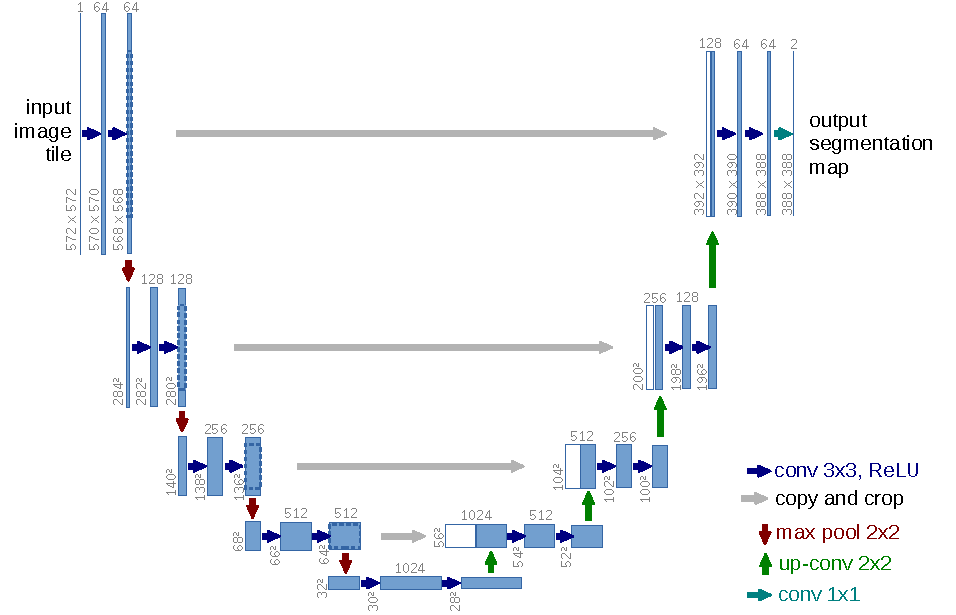
\includegraphics[width=\textwidth]{./Figures/u-net-illustration-correct-scale2.pdf}
	\decoRule
	\caption{The structure of UNet. (Image source:\cite{unet})}
	\label{fig:u-net}
\end{figure}

% why we need a mask
The \textit{U-Net} relies on standard convolutional layers to construct the network. This is useful for image processing tasks with fully dense input data, since there are no missing pixels.
However, for some other input data, such as depth maps acquired by light scanners, it is not always fully dense data, but data with many missing pixels and holes. In this case, we can still apply the standard convolutional layers to extract the feature maps from the semi-dense depth map, but then the valid pixels and the invalid pixels (the missing pixels) will be mixed up during training, resulting in blur and color discrepancy as mentioned by \cite{partial_conv}. Therefore, it is useful to find a way to distinguish the valid and invalid pixels during training. 

\cite{pncnn0} use a binary mask to denote valid pixels, and also use normalized convolution as a surrogate for the default convolutional layer in the training model. The normalized convolution is represented as follows

\begin{equation}
	\begin{array}{rrclcl}
		O(x,y) = 
		\begin{cases}
			\dfrac{\Sigma_i^k\Sigma_j^k W(i,j) \odot I(x-i,y-j) \odot M(x-i,y-j)}{\Sigma_i^k\Sigma_j^k W(i,j) \odot M(x-i,y-j)}, & \text{if}\ \sum_{i}^k\sum_{j}^k M(i,j)>0 \\
			0, & \text{otherwise}
		\end{cases}
	\end{array}
\end{equation}
where $ k $ is the kernel size, $ (x,y) $ is the position in the input, $ (i,j) $ is the displacement in the kennel, and $ M $ is the corresponding mask. A binary mask uses 1 to indicate valid pixels, and 0 otherwise. $ \odot $ denotes element-wise multiplication.



\subsection{Gated Convolution}

% introduce gconv
\cite{gated_activation} proposed a gated activation unit to model more complex interactions compared to standard CNN layers. This was mainly inspired by the multiplicative units that exist in the Long Short-Term Memory (\textit{LSTM}) proposed by \cite{lstm} and the Rated Recurrent Unit (\textit{GRU}) proposed by \cite{gru}. \cite{gconv} has deployed the same gated unit and uses it as a gated convolution layer for training tasks with incomplete input data, such as image inpainting tasks. In this gated convolution layer, the mask used to distinguish between valid and invalid pixels is not specified in advance, but learned during training. The advantage is that the erroneous measurements that are not masked in the depth data can be learned during training to further improve performance. 

The structure is shown in Figure \ref{fig:gconvLayer}. Instead of using a mask as input to indicate valid pixels, a standard convolutional layer is used to learn this mask directly from the data, and a sigmoid function is used as an activation function to indicate the confidence of pixel validation. Meanwhile, another standard convolutional layer is set aside to learn the feature maps with a ReLU/LeakyReLU activation function. Therefore, both the mask and the input features are learned during training.  Then, an element-wise multiplication is performed with the feature map and the mask as the final feature map of this gated convolution layer. 

Formally, the gated convolution is described as follows: the layer with the input $ (N, C_{in}, H, W) $ and the output $ (N, C_{out}, H_{out}, W_{out}) $:

\begin{equation}\label{gconv}
	o(N_i, C_{o_j}) = \sigma(\sum_{k=0}^{C_{in}-1}w_g(C_{o_j}, k) \star i(N_i,k) + b_g(C_{o_j})) * 
	\phi (\sum_{k=0}^{C_{in}-1}w_f(C_{o_j}, k) \star i(N_i,k) + b_f(C_{o_j}))
\end{equation}
where $ \phi $ is the LeakyReLU function, $ \sigma $ is the sigmoid function, so the output values are in the range $ [0,1] $. $ \star $ is the valid 2D cross-correlation operator, $ N $ is the batch size, $ C $ denotes the number of channels, $ H $ is the height of the input planes in pixels, and $ W $ is the width in pixels, $ w(C_{o_j},k) $ denotes the weight of the $ j $-th output channel corresponding to the $ k $-th input channel, $ i(N_i, k) $ denotes the input of the $ i $-th stack corresponding to the $ k $-th input channel, $ b(C_{o_j}) $ denotes the bias of the $ j $-th output channel.


% Gated Convolution Layer
\begin{figure}[H]
	\centering
	\captionsetup{width=\linewidth}
	\begin{tikzpicture}
		\tikzstyle{rect} = [rectangle, rounded corners, minimum width=2.5cm, minimum height=1cm,text centered, draw=black, fill=blue!20]
		\tikzstyle{arrow} = [thick,->,>=stealth]
		\node (output) [rect] {Output};
		\node (oplus) [below of=output, yshift=-.2cm] {$\Huge\odot $};
		\node (LeakyReLU) [rect,below of=oplus, yshift=-0.3cm] {Feature};
		\node (sigmoid) [rect, below of=oplus, yshift=-0.3cm, xshift=-3cm] {Gating};
		
		\node (conv1) [rect,below of=sigmoid, yshift=-1cm] {Gating};
		\node (conv2) [rect,below of=LeakyReLU, yshift=-1cm] {Feature};
		\node (input) [below of=oplus] at (0,-7) {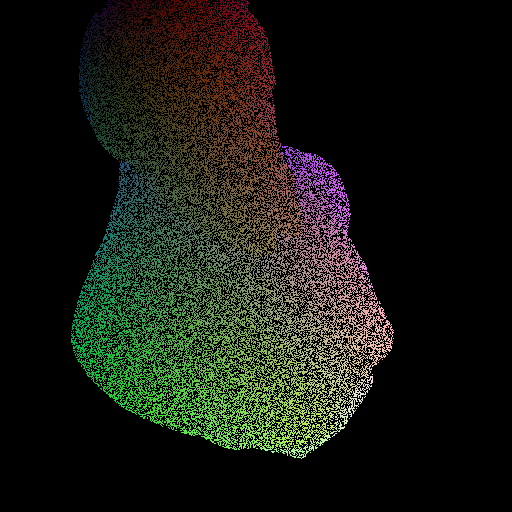
\includegraphics[width=.25\textwidth]{./Figures/train-input.png}};
		
		\draw [arrow] (oplus) -- (output);
		\draw [arrow] (sigmoid) |- (oplus);
		\draw [arrow] (LeakyReLU) -- (oplus);
		
		\draw [arrow] (conv2) --  node [text width=2.5cm, midway, right=1em]{LeakyReLU} (LeakyReLU);
		\draw [arrow] (conv1) --  node [text width=2.5cm, midway, right=1em]{Sigmoid} (sigmoid);
		\draw [arrow] (input) -|  node [text width=2.5cm, midway, below=1em]{Conv2D} (conv1);
		\draw [arrow] (input) -- node [text width=2.5cm, midway, right=1em]{Conv2D} (conv2);
		
		
		
		\node (conv-output) [rect, ] at (6,0) {Output};
		\node (conv-LeakyReLU) [rect,below of=conv-output, yshift=-0.4cm] {Feature};
		\node (conv-conv2) [rect,below of=conv-LeakyReLU, yshift=-1cm] {Feature};
		\node (conv-input) [below of=conv-output] at (6,-7) {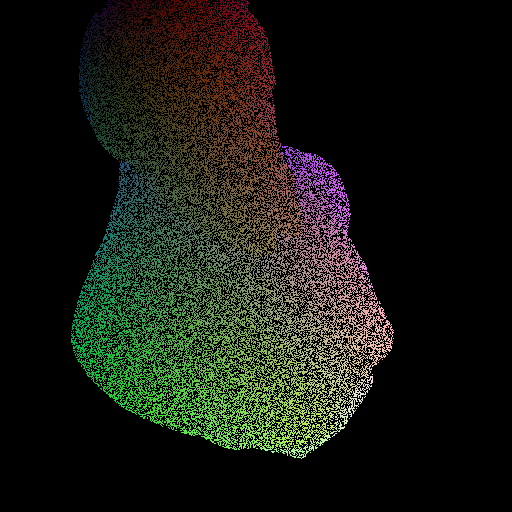
\includegraphics[width=.25\textwidth]{./Figures/train-input.png}};
		
		\draw [arrow] (conv-LeakyReLU) -- (conv-output);
		
		\draw [arrow] (conv-conv2) --  node [text width=2.5cm, midway, right=1em]{LeakyReLU} (conv-LeakyReLU);
		\draw [arrow] (conv-input) -- node [text width=2.5cm, midway, right=1em]{Conv2D} (conv-conv2);
		
		
		
	\end{tikzpicture}
	\decoRule
	\caption{Left: Gated Convolution Layer, where $ \odot $ denotes element-wise multiplication. Right: standard convolution layer.}
	\label{fig:gconvLayer}
\end{figure}


%\section{Canny Edge Detection for Detail Enhancement}
%The inaccuracy part is usually concentrate in the coarse surface or drastic changed surface parts of the object. The corresponding part can be extracted separately via edge detector algorithms, like Canny Edge detector. Feed the edges to a special net for normal prediction might improve the accuracy further. 

\subsection{GCNN Architecture}
\label{sec:architecture}

Based on the above implementation, we proposed a network based on the \textit{U-Net} proposed by \cite{unet}, replacing the standard convolutional layers with gated convolutional layers used for semi-dense normal inference tasks, called gated convolution neural network (\textit{GCNN}), as shown in Figure \ref{fig:gcnn-archi}. 

\begin{sidewaysfigure}[h]
	\centering
	\captionsetup{width=\linewidth}
	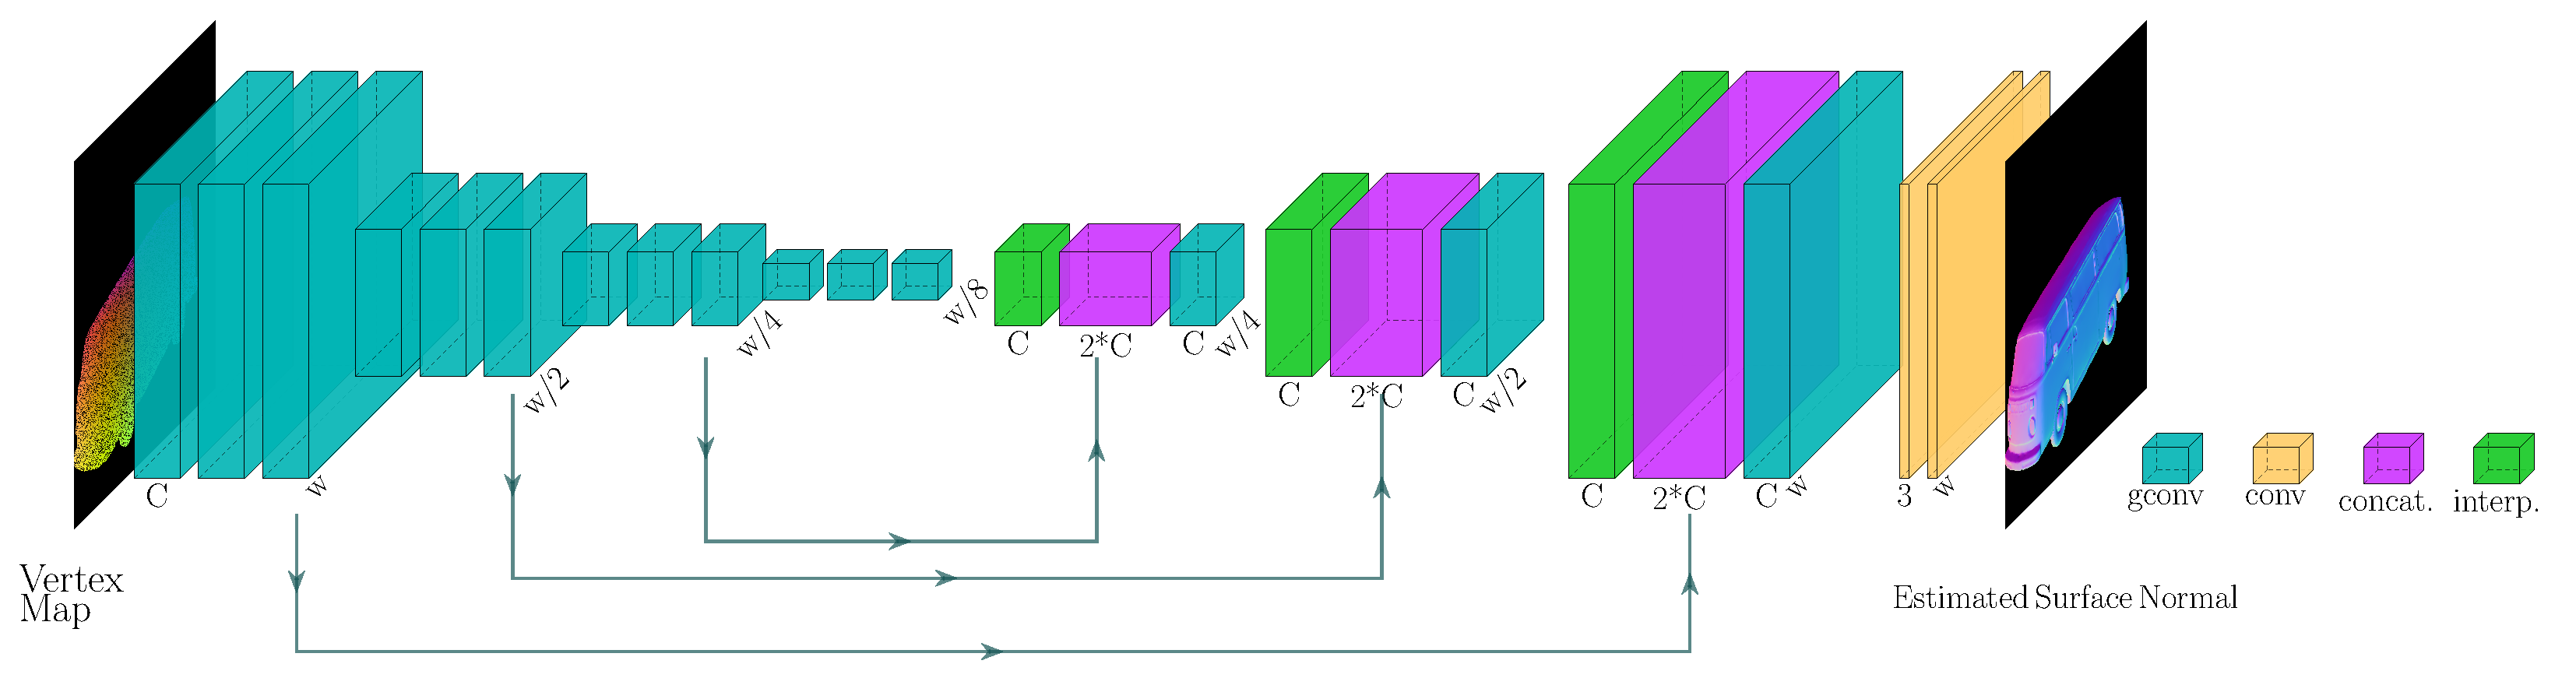
\includegraphics[width=\textwidth]{Figures/gcnn}
	\decoRule
	\caption{The architecture of Gated convolution neural network (\textit{GCNN}) based on Gated convolution and \textit{U-Net} Architecture.}
	\label{fig:gcnn-archi}
\end{sidewaysfigure}

To describe the network in a uniform way, the parameters of the network are represented by letters.
The network consists of a downsampling part and an upsampling part. In the downsampling part, the input has the form $ \textbf{X}_{in} \in \mathbb{R}^{H\times W\times C_{in}}$, while the output is of the form $ \textbf{X}_{out} \in \mathbb{R}^{H\times W\times C_{out}}$
The input matrix goes through 3 down-samples. A down-sampling block consists of two gated convolution layers with stride (1,1) and an additional gated convolution layer with stride (2,2) to reduce the resolution of the feature map. Thus, there are a total of 3 gated convolution layers in each downsampling operation.
The total of three downsamplings extract the geometry features $ \textbf{X}_f $ from the input matrix $ \textbf{X}_{in} $ (represented as regression function $ f $)
\[ f: \textbf{X}_{in} \rightarrow X_f \]
After feature extraction, the network upsamples the feature map three times to obtain the output matrix $ \textbf{X}_{out} $. Each upsampling consists of an interpolation operation that uses nearest neighbor interpolation for upsampling the feature map, and a concatenation layer that concatenates the interpolated result and the corresponding high-resolution feature map $ \textbf{X}_{df_1}, \textbf{X}_{df_2}, \textbf{X}_{df_3} $ from the downsampling part. This is also called a skip connection. In the last step, a gated convolution layer is used to reduce the channel size to fit the next upsampling block. After upsampling three times, the resolution goes back to the original size. After that, two standard convolutional layers without activation function are added to predict the surface normals. The entire upsampling branch can be represented as a regression function $ n $,
\[ n: \textbf{X}_f, \textbf{X}_{df_1}, \textbf{X}_{df_2}, \textbf{X}_{df_3} \rightarrow \textbf{X}_{out} \]
All convolutional layers of the network use the same kernel size $ 3\times 3 $. 


One of the main features of the network is that the output has the same size as the input. This is achieved by (1,1) padding and the same number of channels in the convolution layers. Thus, the surface normal map can be estimated with the same dimension as input data. Another important point of the network is its robustness to noise using gated convolutional layers. The network can take a semi-dense matrix as input and then predict the fully dense matrix as output. The last feature is the multipurpose use of scenarios. No specific input type is given in the description. 
The network is also fully convolutional and therefore can accept different input resolutions. 


\section{Illuminated Calibrated RGB-D Image based Normal Inference}
\label{sec:trip-net}
The GCNN architecture is designed for one type of input, since it has only one pipe to process the data. In our work, the input refers to a structured point cloud. Therefore, it is suitable for a geometry-based approach that uses the point cloud as input and estimates the corresponding surface normal. However, as mentioned in the introduction, the goal of this work is to discuss the improvement of normal inference based on an illuminated calibrated RGB-D image, i.e., we want to see if we can improve the performance of normal estimation not only based on geometry information such as the point cloud or the depth map, but also with illumination information such as the image and the light map. Therefore, we need to find an architecture that takes into account all these types of data. 


\subsection{Light Map, Gray-scale Image and Vertex Map}
\label{sec:lightmap}
First, we present the required input types for our network.

\paragraph{Vertex Map}
The vertex map $ \textbf{V} $ is converted from the depth map presented in chapter \ref{ch:04}, while the depth map is acquired from a depth camera. It contains a set of surface point locations in 3D space. Each pixel in the vertex map corresponds to a point position. These vertices contain the geometry information of the object surface, which can be further used for training deep learning models. For each scene, the camera takes only one image, leaving only one vertex map. However, as mentioned earlier, the vertex map is only semi-dense. We use such a semi-dense vertex map as input for the surface normal estimation.

\paragraph{Grayscale Image}
The grayscale image $ \textbf{I} $ is acquired in correspondence with the depth map using the same calibrated camera equipment, so the intrinsic matrix $ \textbf{K} $ and the extrinsic camera matrix $ [\textbf{R}|\textbf{t}] $ are known. Unlike the vertex map, it is usually completely dense.

\paragraph{Light Map}
The light map $ \textbf{L} $ can be derived from the vertex map $ \textbf{V} $. The position of the light source $ (s_x, s_y, s_z) $ is given by the input data. As shown in Figure \ref{fig:lambertian-surface}, the direction of the incident light is a vector point from the light source to the surface point and can therefore be calculated as follows.

\begin{equation}\label{light-direction}
	\begin{array}{ll}
		\textbf{L}(x,y,z)&= \dfrac{\textbf{V}(x,y,z)-(s_x,s_y, s_z)}{\|\textbf{V}(x,y,z)-(s_x,s_y, s_z)\|_2}\\ 
	\end{array}
\end{equation}
where both $ (s_x, s_y, s_z) $ and $ \textbf{V} $ refer to the camera space. The light direction map $ \textbf{L} $ is normalized since only the direction of the light is considered. Applying the above equation for all pixels in the point cloud, we obtain the corresponding light map, which is a matrix with the same size as the point clouds. However, it should be noted that the light map is calculated based on the vertex map, while the vertex map in the training pipeline is only semi-dense, so the light map is also semi-dense and has the same noise feature as the vertex map, as shown in Figure \ref{fig:light-input}. 

\begin{figure}[H]
	\centering
	\captionsetup{width=\linewidth}
	{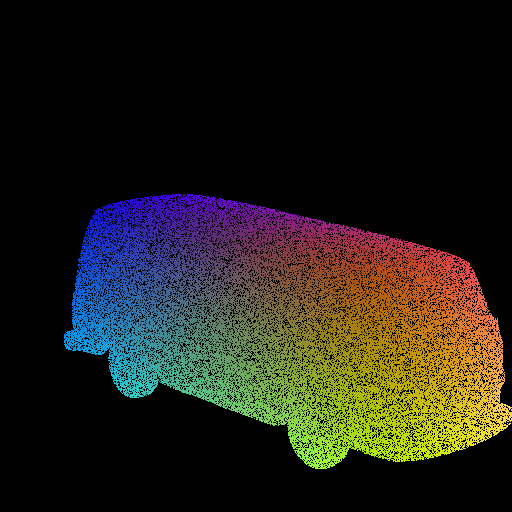
\includegraphics[width=.32\textwidth]{./Figures/intrinsic_image_vertex_input.png}}
	{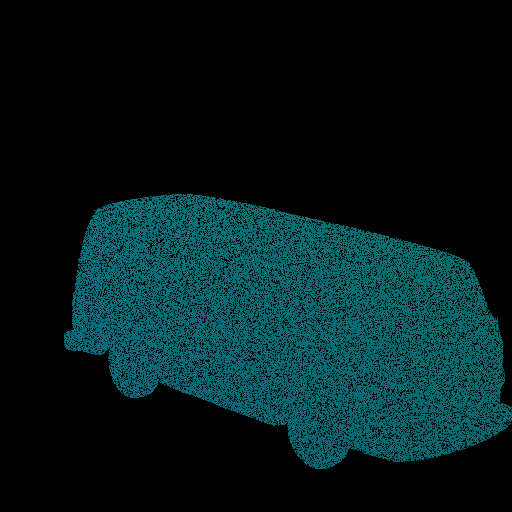
\includegraphics[width=.32\textwidth]{./Figures/intrinsic_image_light_input.png}}
	{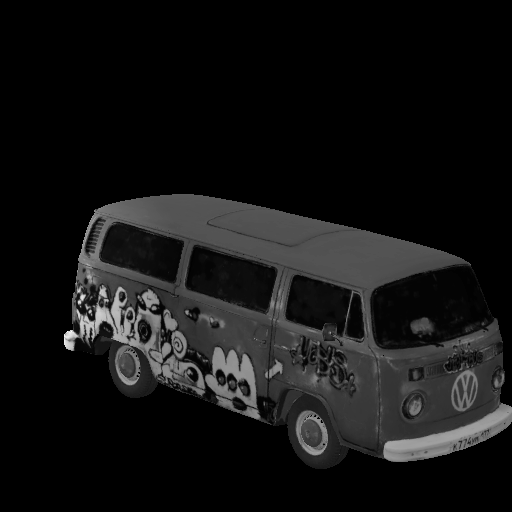
\includegraphics[width=.32\textwidth]{./Figures/intrinsic_image.png}}
	\decoRule
	\caption{Three kinds of input data. From left to right, vertex map, light map, gray-scale image.}
	\label{fig:light-input}
\end{figure}
See chapter \ref{ch:04} for more details on how to set up the dataset.


%\subsection{VIL Net}
%Based on above implementations, we propose a light and image guided network called Vertex-Image-Light Network (VIL-Net). The structure is basically derived from GCNN model as mentioned in \ref{sec:gcnn}, which is shown in Figure 
%\ref{fig:VIL-Net}.
%
%As mentioned in the name, the \textbf{VIL}-Net utilizes \textbf{V}ertex map, \textbf{L}ight map and \textbf{I}mage map to accomplish the normal inference task. 
%
%The network can be consider in two parts. The first part extracts the feature maps from the input data. It deals with two kinds of input, the vertex map $ X_1 \in \mathbb{R}^{w\times h\times3}$, and the concatenation of light and image map $ X_2 \in \mathbb{R}^{w\times h\times4} $. The network extracts the geometry features $ X_v $ from vertex map $ X_1 $ (represented as a regression function v)
%\[ v: X_1 \rightarrow X_v \]
%and the photometric features $ X_l $ from image and the light map $ X_2 $ (represented as a regression function $ l $)
%\[ l: X_2 \rightarrow X_l \]
%where the two encoders have the same network architecture based on the downsampling part of GCNN model. After the feature extraction, 2 extra layers are added: 1, a concatenate layer is added to fuse the vertex feature, and the image and light map feature getting from the encoder. 
%2, a fused feature map is predicted from all the feature maps base on a single gated convolution layer. (represented as a regression function $ m $)
%\[ m: [X_v X_l] \rightarrow X_f \]
%Then the network interpolates the feature maps $ X_f $ 3 times using interpolation and gated convolution layers to inference the normal map $ N $. Meanwhile, the skip connections fuse the high resolution features $ X_{df_1, df_2, ...} $ from the downsampling part during the upsamplings. The upsampling is represented as a regression function $ n $:
%\[ n: X_f, X_{df_1, df_2, ...} \rightarrow N \]
%
%With the help of an extra image-light encoder, the network gained more information of the object surface, which is supposed to predict the surface normal more accurate. In this scenario, the output is still the surface normal, thus the training loss can be the same as GCNN model.


\subsection{Trip-Net Architecture}
We proposed a network that considers the vertex map, the light map, and the grayscale image for surface normal inference, which is called the Triple-Pipe-Gated Network (\textit{Trip-Net}). 
The \textit{Trip-Net} uses the GCNN architecture three times to perform the normal inference task, so we call it \textit{Triple-Pipe-Gated}. The architecture is shown in Figure \ref{fig:Trip-Net}.

The network consists of three pipes combined with one main pipe and two side pipes. Each pipe deals with a different task. The Main Pipe deals with the geometry information, which takes the vertex map as input and is used to predict the surface normal. The light map takes a Side Pipe as input, from which the light features are extracted and then passed to the Main Pipe as additional information for normal estimation. The image map takes another Side Pipe to extract the image features, and then forwards the features to the Main Pipe as well. The additional pipes provide the illumination information that helps the Main Pipe refine the inferred normals.

\paragraph{Side-Pipe (Light)}
 The structure of the Light-Pipe is almost identical to the architecture of the GCNN. It takes the light map $ \textbf{L} \in \mathbb{R}^{W\times H\times 3}$ as input and then passes through gated convolution layers three times to obtain the feature maps,
 $ \textbf{X}_{L1D} \in \mathbb{R}^{{W}\times H\times C} $,
 which has the same resolution as the input map.
 Then three downsampling operations are followed afterwards. In each downsampling, 3 gated convolution layers are used to further extract the feature maps, where the first two gated convolution layers have stride (1,1) and the third gated convolution layer has stride (2,2). Then we get
  
$ \textbf{X}_{L2D} \in \mathbb{R}^{\frac{W}{2}\times \frac{H}{2}\times C} $,
$ \textbf{X}_{L3D} \in \mathbb{R}^{\frac{W}{4}\times \frac{H}{4}\times C} $,
$ \textbf{X}_{L4D} \in \mathbb{R}^{\frac{W}{8}\times \frac{H}{8}\times C} $
(represented as a regression function $ l_{down} $)
\[ l_{down}: \textbf{L} \rightarrow  \textbf{X}_{L1D} , \textbf{X}_{L2D}, \textbf{X}_{L3D}, \textbf{X}_{L4D} \]
For the up-sampling operation, it takes 3 times up-sampling to generate higher resolution light feature maps
$ \textbf{X}_{L1U} \in \mathbb{R}^{{W}\times {H}\times C} $,
$ \textbf{X}_{L2U} \in \mathbb{R}^{\frac{W}{2}\times \frac{H}{2}\times C} $,
$ \textbf{X}_{L3U} \in \mathbb{R}^{\frac{W}{4}\times \frac{H}{4}\times C} $ respectively, whereas each up-sampling also considers the feature maps in the down-sampling part,
(represented as a regression function $ l_{up1}, l_{up2}, l_{up3} $)
\[ 
\begin{matrix}
	l_{up3} : \textbf{X}_{L3D}, \textbf{X}_{L4D} \rightarrow \textbf{X}_{L3U} \\
	l_{up2} : \textbf{X}_{L2D}, \textbf{X}_{L3U} \rightarrow \textbf{X}_{L2U} \\
	l_{up1} : \textbf{X}_{L1D}, \textbf{X}_{L2U} \rightarrow \textbf{X}_{L1U} \\
\end{matrix}
\]
In our network, each up-sampling is done in three layers, an interpolation layer based on the nearest neighbor algorithm, a concatenation layer to concatenate the interpolated feature maps and the corresponding feature maps in the down-sampling part, and a gated convolution layer to reduce the channel size.
The light pipe branch is completed in the last layer of the third up-sampling.

In this branch, four kinds of feature maps $ \textbf{X}_{L4D}, \textbf{X}_{L3U}, \textbf{X}_{L2U}, \textbf{X}_{L1U} $ are used as guided information for further operation.

\paragraph{Side-Pipe (Image)}

The task of the Image-Pipe in the network is to predict the image features. This pipe is a pipe cooperating with the Light-Pipe. The architect is the same as that of the Light-Pipe, but only the input is the image matrix $ \textbf{I}\in \mathbb{R}^{W\times H\times 1}$. The first set of the feature maps are $ \textbf{X}_{I1D} \in \mathbb{R}^{{W}\times H\times C} $, noting that it has the same channel as the light feature maps. Then, the down-sampling is performed three times to extract the image feature maps

$ \textbf{X}_{I2D} \in \mathbb{R}^{\frac{W}{2}\times \frac{H}{2}\times C} $,
$ \textbf{X}_{I3D} \in \mathbb{R}^{\frac{W}{4}\times \frac{H}{4}\times C} $,
$ \textbf{X}_{I4D} \in \mathbb{R}^{\frac{W}{8}\times \frac{H}{8}\times C} $
(represented as a regression function $ i_{down} $)
\[ l_{down}: \textbf{I} \rightarrow  \textbf{X}_{I1D} , \textbf{X}_{I2D}, \textbf{X}_{I3D}, \textbf{X}_{I4D} \]
It requires three times upsampling to produce higher resolution image feature maps.
$ \textbf{X}_{I1U} \in \mathbb{R}^{{W}\times {H}\times C} $,
$ \textbf{X}_{I2U} \in \mathbb{R}^{\frac{W}{2}\times \frac{H}{2}\times C} $,
$ \textbf{X}_{I3U} \in \mathbb{R}^{\frac{W}{4}\times \frac{H}{4}\times C} $ respectively, whereas each up-sampling also considers the feature maps in the down-sampling part,
(represented as a regression function $ i_{up1}, i_{up2}, i_{up3} $)
\[ 
\begin{matrix}
	i_{up3} : \textbf{X}_{I3D}, \textbf{X}_{I4D} \rightarrow \textbf{X}_{I3U} \\
	i_{up2} : \textbf{X}_{I2D}, \textbf{X}_{I3U} \rightarrow \textbf{X}_{I2U} \\
	i_{up1} : \textbf{X}_{I1D}, \textbf{X}_{I2U} \rightarrow \textbf{X}_{I1U} \\
\end{matrix}
\]
whereas the layers in the upsampling part have the same architecture as the Light Pipe. In the Image Pipe, four types of feature maps $ \textbf{X}_{I4D}, \textbf{X}_{I3U}, \textbf{X}_{I2U}, \textbf{X}_{I1U} $ are used as guided information for further operation.


\paragraph{Main-Pipe (Vertex)}
The task of the vertex pipe in the network is to predict the normal map directly, also taking into account the feature maps in the other channels. The input is the vertex map $ \textbf{V} \in \mathbb{R}^{W\times H\times 3}$ converted from the point cloud. 
The downsampling part is still the same as for the other two pipes. The feature maps in each downsampling part are of the form
$ \textbf{X}_{V1D} \in \mathbb{R}^{{W}\times H\times C} $, 
$ \textbf{X}_{V2D} \in \mathbb{R}^{\frac{W}{2}\times \frac{H}{2}\times C} $,
$ \textbf{X}_{V3D} \in \mathbb{R}^{\frac{W}{4}\times \frac{H}{4}\times C} $,
$ \textbf{X}_{V4D} \in \mathbb{R}^{\frac{W}{8}\times \frac{H}{8}\times C} $, respectively, 
(represented as a regression function $ i_{down} $)
\[ v_{down}: \textbf{V} \rightarrow  \textbf{X}_{V1D} , \textbf{X}_{V2D}, \textbf{X}_{V3D}, \textbf{X}_{V4D} \]
The up-sampling operation has a different situation than the other two pipes.
It merges the output feature maps with the corresponding resolution from three pipes to get a merged feature map 
$ \textbf{X}_{F3U} \in \mathbb{R}^{W\times H\times C} $, 
$\textbf{X}_{F2U} \in \mathbb{R}^{W\times H\times C} $, 
$\textbf{X}_{F1U} \in \mathbb{R}^{W\times H\times C} $,
in each up-sampling stage, (represented as regression functions $ f_{up1}, f_{up2}, f_{up3}, f_{up4}$)
\[ 
\begin{matrix}
	f_{up4} : \textbf{X}_{I4D}, \textbf{X}_{L4D}, \textbf{X}_{V4D} \rightarrow \textbf{X}_{F4U} \\
	f_{up3} : \textbf{X}_{I3U}, \textbf{X}_{L3U}, \textbf{X}_{F4U} \rightarrow \textbf{X}_{F3U} \\
	f_{up2} : \textbf{X}_{I2U}, \textbf{X}_{L2U}, \textbf{X}_{F3U} \rightarrow \textbf{X}_{F2U} \\
	f_{up1} : \textbf{X}_{I1U}, \textbf{X}_{L1U}, \textbf{X}_{F2U} \rightarrow \textbf{X}_{F1U} \\
			
\end{matrix}
\]
Each upsampling consists of 5 layers: An interpolation layer to double the resolution using the nearest interpolation algorithm, a gated layer to reduce the channel size to 1/3 of itself for inter-pipes feature reduction, a concatenation layer to connect the output with the corresponding feature map in the downsampling part (skip connection), a gated layer to reduce the channel size to 1/2 of itself for skip-connection feature reduction, a concatenation layer to merge the corresponding upsampling feature map from the other two pipes with the feature map in the current pipe altogether. These 5 layers take into account both the information from the other pipes and the feature maps from the downsampling part. 

At the end of the network, to fit the task of normal inference, two standard convolutional layers are added to convert the normal map $ \textbf{X}_{N} \in \mathbb{R}^{\frac{W}{8}\times \frac{H}{8}\times 3} $ (represented as a regression function $ n $)
\[n:\textbf{X}_{F1U} \rightarrow \textbf{X}_{N} \] 

\begin{sidewaysfigure}[h]
	\centering
	\captionsetup{width=\linewidth}
	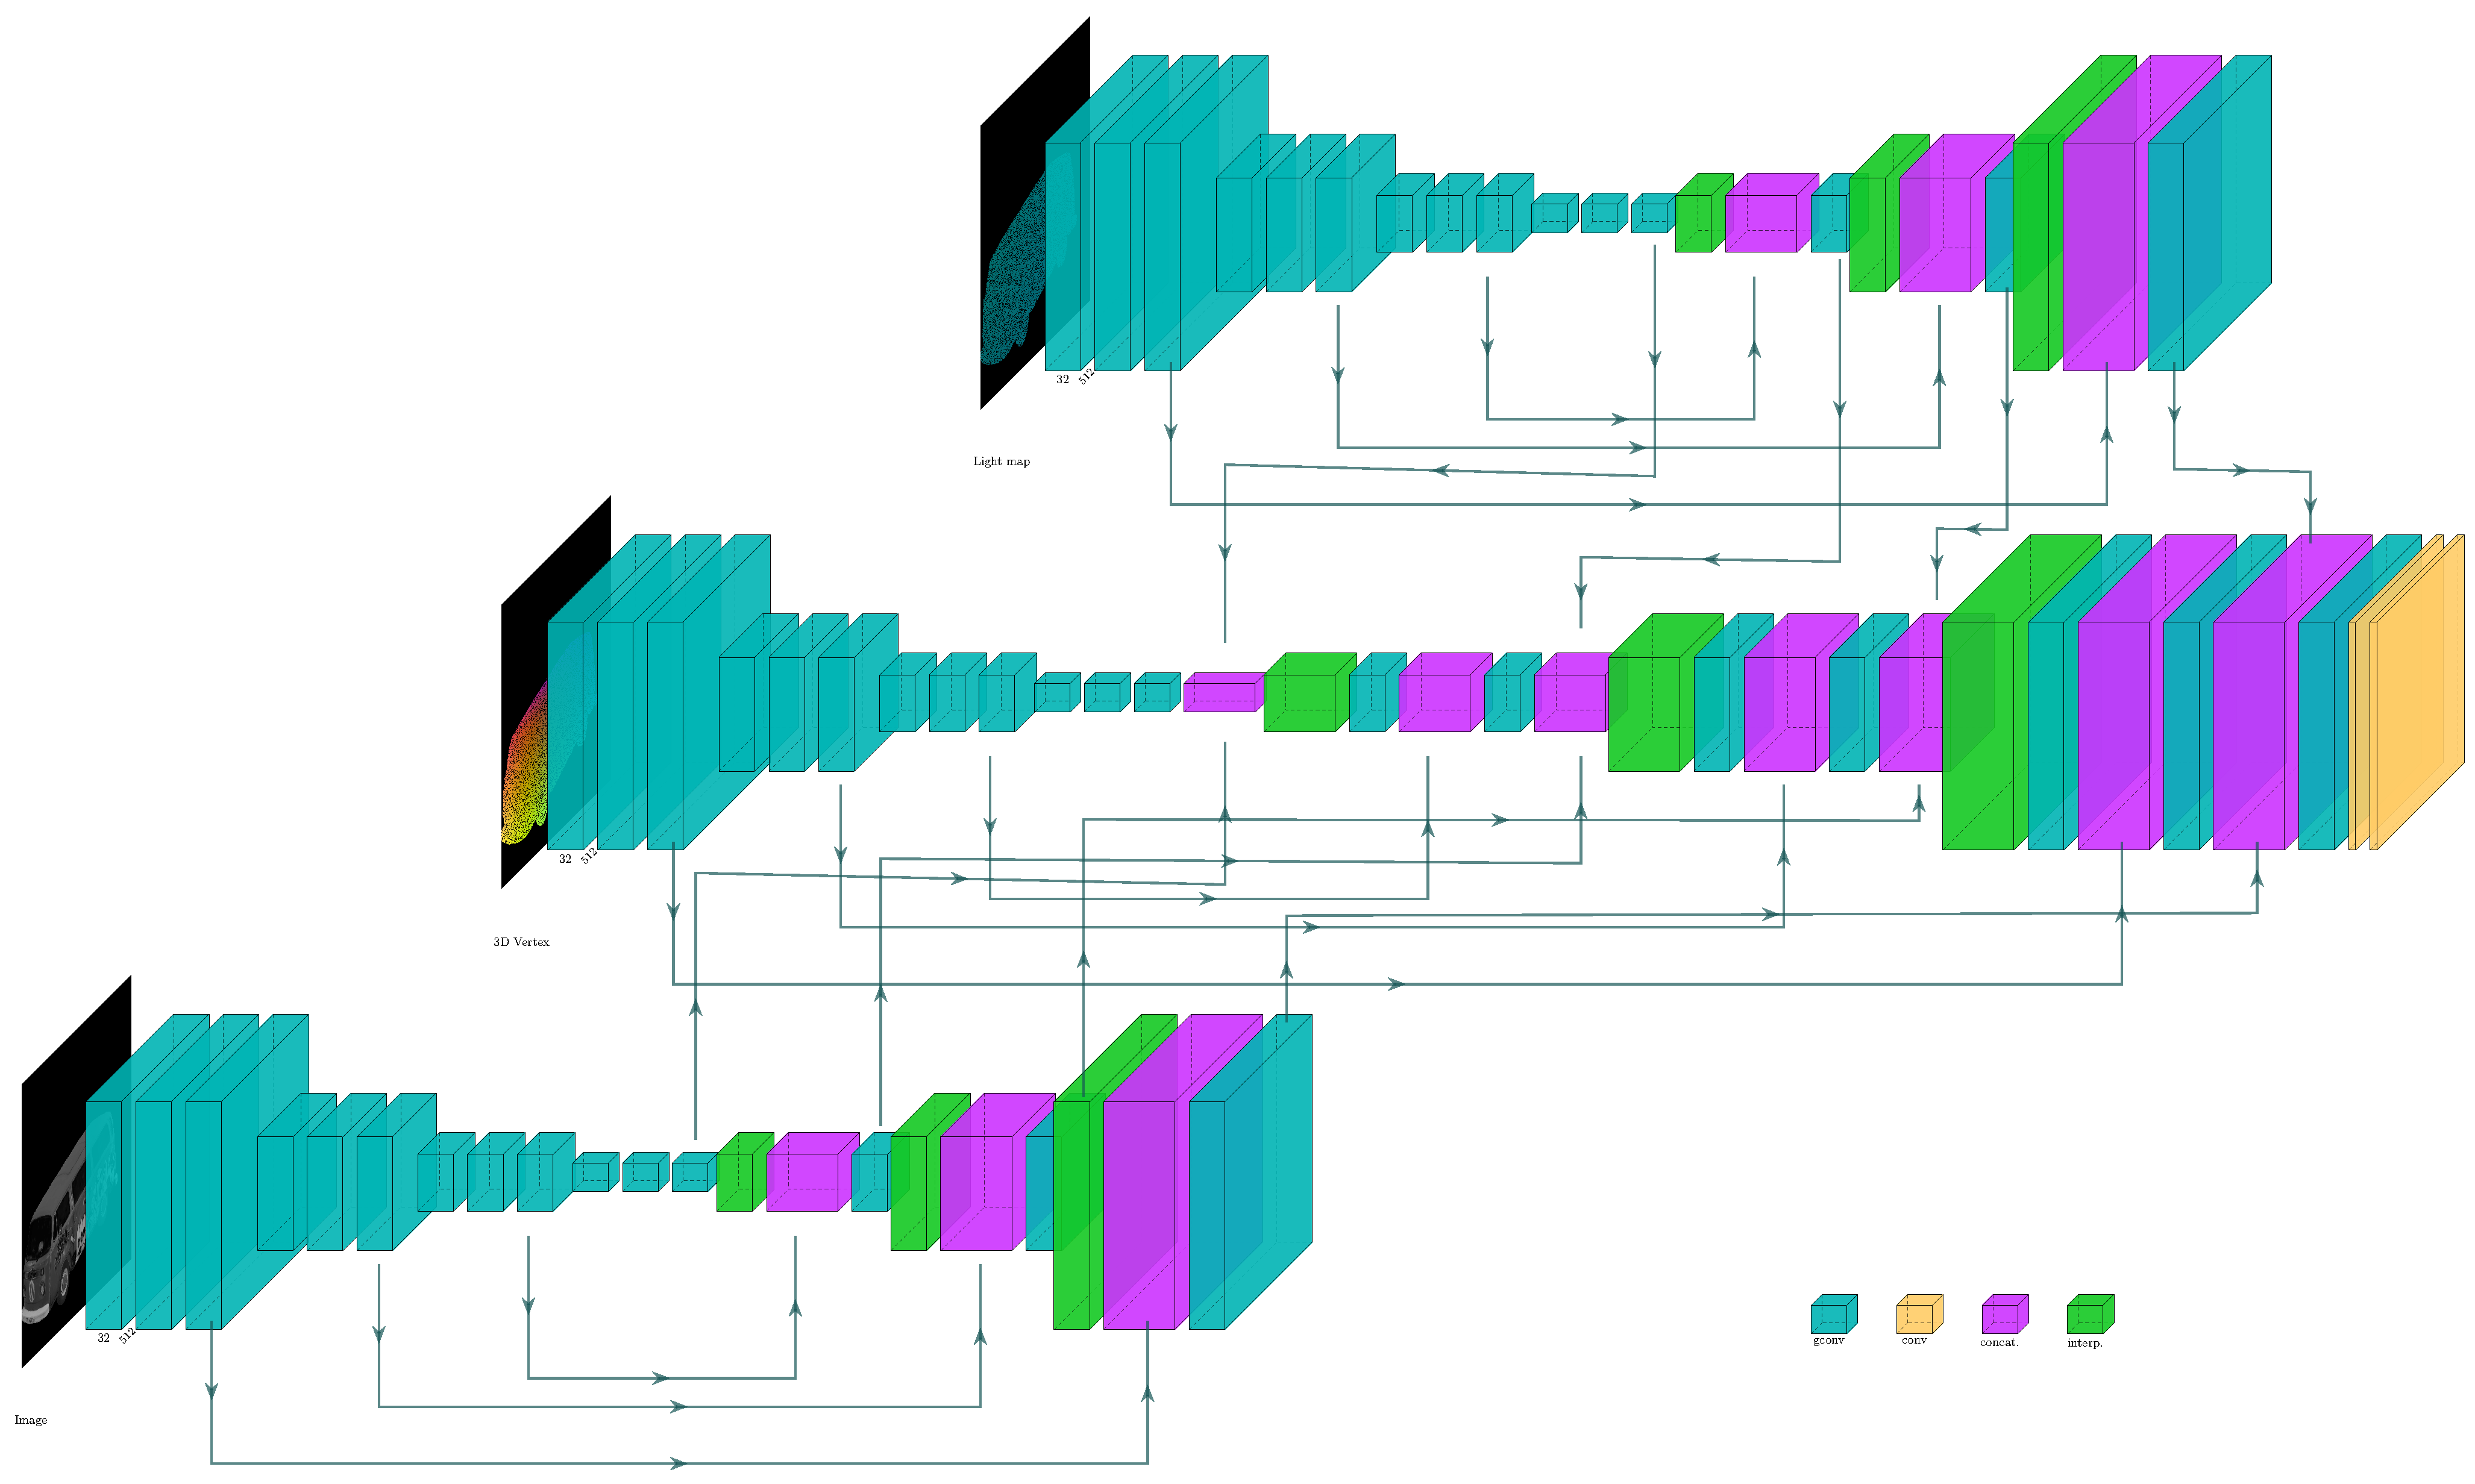
\includegraphics[width=\textwidth]{Figures/trignet} % Research group name and department name
	\decoRule
	\caption{The architecture of the \textit{Trip-Net}.}
	\label{fig:Trip-Net}
\end{sidewaysfigure}



%% loss function 

\subsection{Loss Functions}
We have investigated different loss functions for training our network. The most common loss functions are the L1 loss and the L2 loss for image simulation. In our experiments, we used a modified Huber loss function to train our model, which yields a lower error in the evaluation compared to a pure L1 or L2 loss function. 

\paragraph{L1 Loss}
L1 loss, also known as absolute error loss, which calculates the absolute difference between the prediction and the ground truth. It leads to the mean value of the absolute errors of the observations.
\[ L_1(\tilde y - y) = |\tilde y - y | \]

\paragraph{L2 Loss}
The standard loss function for optimization in regression problems is the L2 loss, also known as squared error loss, which minimize the squared difference between a prediction and the actual value. It leads to the mean of the observations. 
\[ L_2(\tilde y - y) = \|\tilde y - y \|_2^2 \]


%\paragraph{Masked L2 Loss with penalty for outliers(mask-l2)}
%\label{par:maskl2}
%The background pixels of the input data are not considered in the normal inference task, they are saved as black pixels in the input data. These pixels should not considered in the loss function, i.e. invalid pixels. Therefore, a valid mask is required to distinguish the background and the main object. Specifically, using a matrix with the same width and height as the output, for each pixel, 0 is invalid, 1 is valid. 
%Furthermore, depends on the specific task, the output should be constraint in a range. For normal output, the range is $ [-1,1] $. Thus for the outliers out of this range, a outlier mask can be applied to give them a penalty.
%
%\begin{equation}\label{gcnn-loss}
%	\begin{array}{ll}
%		l(x,y)&= L  = \{l_1, ..., l_N\}^T\\ 
%		l_{n\in N} &= \| mask_{obj} \odot mask_{ol} \odot ( {\tilde y}_n - y_n) \|_2^2 + 	\| mask_{obj} \odot mask_{nol} \odot ( {\tilde y}_n - y_n) \|_2^2 \\
%	\end{array}
%\end{equation}
%
%where $ x $ is input, $ y $ is target, $ N $ is the batch size.$ mask_{obj} $ is the mask of the object, i.e. 1 means it is an pixel on the object, 0 is an pixel on the background. $ mask_{ol} $ is the mask for the outliers, i.e. 1 means outliers, 0 means non outlier, $ mask_{nol} $ is exactly the inverse of $ mask_{ol} $. $ p $ is the penalty of the outliers, it is set as 1.4.


\paragraph{Huber Loss}
Inspired by \cite{img2depth}, we use the Huber loss provided by \cite{berhu-loss} for our model training, which indeed achieves a better error than a simple L2 loss. It can be described mathematically as follows.


\begin{equation}\label{berhu-loss}
	\begin{array}{ll}
		\mathcal{B}(y)= \begin{cases}
			|y| & |y| \ge c \\
			\dfrac{y^2 + c^2}{2c} & |x| < c\\
		\end{cases}
	\end{array}
\end{equation}
where $ c=0.2\max (|\tilde y - y|) $. The shape of the loss is shown in Figure \ref{fig:berhu-loss-shape}. Huber loss is a combination of L1 and L2 loss, being L2 loss in the range $ [-c,c] $ and L1 loss outside this range. The loss is also differentiable at the junction of two first order intersection functions. As mentioned in \cite{img2depth}, the parameter $ c=0.2 \max(|\tilde y - y|) $ corresponds to the 20\% of the maximum error per batch. 

\begin{figure}[H]
	\centering
	\captionsetup{width=\linewidth}
	\begin{tikzpicture}
		\pgfplotsset{ticks=none}
		\begin{axis} [axis lines=center]
			\addplot [domain=1:2, smooth, thick, width=5mm, color=red] { x };
			\addplot [domain=0:1, smooth, width=5mm] { x };
			\addplot [domain=-1:0, smooth, width=3mm] { -x };
			\addplot [domain=-2:-1, smooth, thick, width=3mm, color=red] { -x };
			\addplot [domain=-1:0, smooth, thick, color=red] { (x^2+1^2)/(2*1) };
			\addplot [domain=0:1, smooth, thick, color=red] { (x^2+1^2)/(2*1) };
		\end{axis}
	\end{tikzpicture}
	\caption{The shape of Huber Loss (show in red line). }
	\label{fig:berhu-loss-shape}
\end{figure}


